\section{Approach}
\label{sec:method}

%In this section, we first present the three-stage pipeline method and filtering method, then we will introduce our joint model for QA pairs generation.
In this section, we present the structure of the pipeline method and filtering method for generating aspect focused QA pairs from the document. 
%\ZL{Change the "hint" in the pictures to "aspects"}

\subsection{Pipeline Method}
\label{sec:pipeline}
The task is to generate several question-answer pairs (QA pairs) with the input of document $D=\{P_1, P_2, ... , P_n\}$ and aspect $Aspect$, it can be divided into three steps shown in Figure~\ref{fig:pipeline}: Paragraph Retrieval, Answer Extraction and Question Generation. In the pipeline method, all steps are trained separately.
\paragraph{Paragraph Retrieval.} The reason we need to retrieve paragraphs from documents is that documents are too long as an input of any deep learning models. 

In this step, we choose the paragraphs with higher relevance to aspect.
%The retrieval methods such as TF-IDF and BM25 are chosen to select the relevant paragraph list.
%The pre-trained model BERT are also 
For each document, the input of the retrieval model is a list of paragraphs $[P_1, P_2, \cdot\cdot\cdot]$ and the aspect $Aspect$, and the output is a ranked list of paragraphs with their aspect-paragraph relevance scores.
%The input is a list of documents $[D_1, D_2, \cdots]$ and the aspect, and the output is a list of (paragraph, aspect) pairs $[PA_1, PA_2, \cdots]$. 
%We split the documents into paragraphs first, for each paragraph, we use a two-class classifier to judge whether it is relevant to the aspect. We use three methods for this step in our framework, they are 
%\ZL{[Add ref here]}
%TF-IDF scores with threshold, BM25 scores with threshold and Bert classifier. 

We choose two traditional rule-based methods TF-IDF and BM25~\cite{robertson2009probabilistic} to get the relevant paragraphs.
Due to the remarkable effect of pre-trained models, we also implement a BERT classifier to do the paragraph ranking\cite{qiao2019understanding}.
The input of BERT is a $(P_i, Aspect)$ pair and the output which can be regarded as the relevance score is the positive confidence of the [CLS] token after a classification layer.

%The former two methods are traditional rule-based methods to calculate the relevance between a document and a word or phrase, and the later is used in many tasks in recent years due to its remarkable effect.
\paragraph{Answer Extraction.} In this task, the answer is exactly extracted from the document, while the question needs to be generated. So we choose to extract answers first. 

Follow the work of Subramanian et al.~\shortcite{subramanian2017neural}, we use two methods, entity tagging (NER), and pointer network, to extract answers.
The input is $(P_i, Aspect)$ pair from retrieval. For entity tagging, we use the spaCy\footnote{https://spacy.io/docs/usage/entity-recognition} to predict entities in $P_i$ and keep all entities. For the pointer network, it will generate all possible answer positions of $P_i$. We implement pointer network as Subramanian et al's~\shortcite{subramanian2017neural}. 
%Considering that the error of this step will continue to the next step,
%while generating the question according to (paragraph, answer) pairs and generating the answer according to (paragraph, question) pairs are both hot research fields. 
%we choose to generate answers first because we can extract answers from paragraphs instead of generating them, and extraction generally causes less error than a generation.

We also tried the sequence labeling method. The BIO tagging model implemented by BiLSTM-CRF predicts ``O" for every token. We think the reason is the answer is too sparse in each $P_i$, which misleads the model to predict ``O'' for every token. So we split $P_i$ into sentences $\{S_{i,1}, S_{i,2}, ..., S_{i,n}\}$ and use tagging model to predict BIO tagging for each $S_{i,j}$. Finally, we combine all the sentence tagging as the tagging of $P_i$.

We don't use $Aspect$ information in this step because the relevance between aspect and answers is not strong. We randomly sample some samples from the training data. Only 34\% aspects are relevant to the answer. For example in the paragraph about Black Death:
%\begin{equation*}
%\begin{aligned}
%&{\rm Q:\ When\ did\ the\ plague\ return\ to\ Europe?}\\
%&{\rm A:\ throughout\ the\ 14th\ to\ 17th\ centuries}\\
%&{\rm Aspect:\ Recurrence}\\
%\end{aligned}
%\end{equation*}
\begin{equation*}
\begin{aligned}
&{\rm Q:\text{\ When\ did\ the\ plague\ return\ to\ Europe?}}\\
&{\rm A:\text{\ throughout\ the\ 14th\ to\ 17th\ centuries}}\\
&{\rm Aspect:\text{\ Recurrence}}\\
\end{aligned}
\end{equation*}

The $Aspect$ is relevant to the QA pair but it's not relevant to A directly. Different from answer extraction, for question generation in more than half (about 56\%) samples aspect, is directly relevant to the Q. So we use aspects to help the model to generate more relevant questions. The results in the experiment show the aspect information is important in question generation step.
%For each (paragraph, aspect) pair $PA_i$ generated in the former step, we extract some spans from the paragraph as answers. This is a sequence labeling problem, for each token, it can be ``not in an answer'' (O-Ans), ``begin of an answer'' (B-Ans) or ``in an answer'' (I-Ans). We extract answers from the input (paragraph, aspect) pairs to form (paragraph, aspect, answer) triples. Note that a ``[SEP]'' token is used to split the input paragraph and aspect in this step, and the label for the sequence is only for the paragraph segment. In this step, we try the following three methods: \ZL{[Add ref here]} 
%take NER as answer spans, Bi-LSTM+CRF, and Pointer Network. Many extracted answers are name entities, so we take NER as one of the extraction methods. We also take Bi-LSTM+CRF and Pointer Network since they are well-known for their significant effects on sequence labeling tasks.
\paragraph{Question Generation.} Generating questions given paragraphs and answers is a hot research topic, but different from the traditional Question Generation tasks, we not only take the paragraph and the answer as input to generate a question, but also take the aspect. The input triple is $(P_i, Aspect, A)$, where $A=\{a_1,a_2,...,a_m\}$ is the extracted answer list. We implement this based on two question generation models. One is seq2seq model~\cite{zhao2018paragraph}. This model uses RNN and gets self-attention to encode the paragraph and use another RNN to generate words sequence with copy mechanism. To restrict the generated question with the aspect, we use another LSTM encoder for the aspect. Then use attention to aggregate information from aspect to the paragraph.
\begin{equation}
\begin{aligned}
u_{p} &= LSTM(e_{p}, m_{p}) \\
u_{a} &= LSTM(e_{a}) \\
u_{p} &= gated\ attention(u_{a}, u_{p})\\
\end{aligned}
\end{equation}
Where $e_p$ and $e_a$ is the word embedding representation of  $P_i$ and $Aspect$. $m_p$ is the meta-word representation which identifies whether each word in the paragraph is in or outside the answer in $A$. The others are the same as the original model.

Another one is UNILM model~\cite{dong2019unified}. UNILM is the SOTA method for Question Generation, it realizes this task with the help of a language model which trained with the combination of uni-direction, bi-direction, and seq2seq. Similar to the answer extraction step, for each input triple, we combine the three segments in the same sequence as the first segment of UNILM and use ``[SEP]'' tokens to split paragraph, aspect and answer:

\begin{equation*}
\begin{aligned}
{\rm P_i\ [SEP]\ Aspect\ [SEP]\ a_i}\\
\end{aligned}
\end{equation*}
where $a_i$ is an answer in $A$. And the second segment is the generated question.
 
In this step, given triple $(P_i, Aspect, A)$, we will generate question list $Q$ according to the $A$, and we take the generated questions and the input answers as generated QA pairs. 

% In this part, we design a three-step pipeline structure which is shown as Figure \ref{fig:pipeline}. All steps are trained separately.

% %In this part, the answers are extracted from the source 
% \textbf{Paragraph Retrieval.} Two different methods are used here to select valid paragraphs with high relevance to the hint from the document.

% \textbf{Answer extraction.} Answers exist in the source document. The extraction module uses the approach of sequence labeling to mark the position of answers.

% \textbf{Question generation.} Question generation module is to generate questions from the document and a relevant answer span.

\begin{figure}[th]
    \begin{center}
    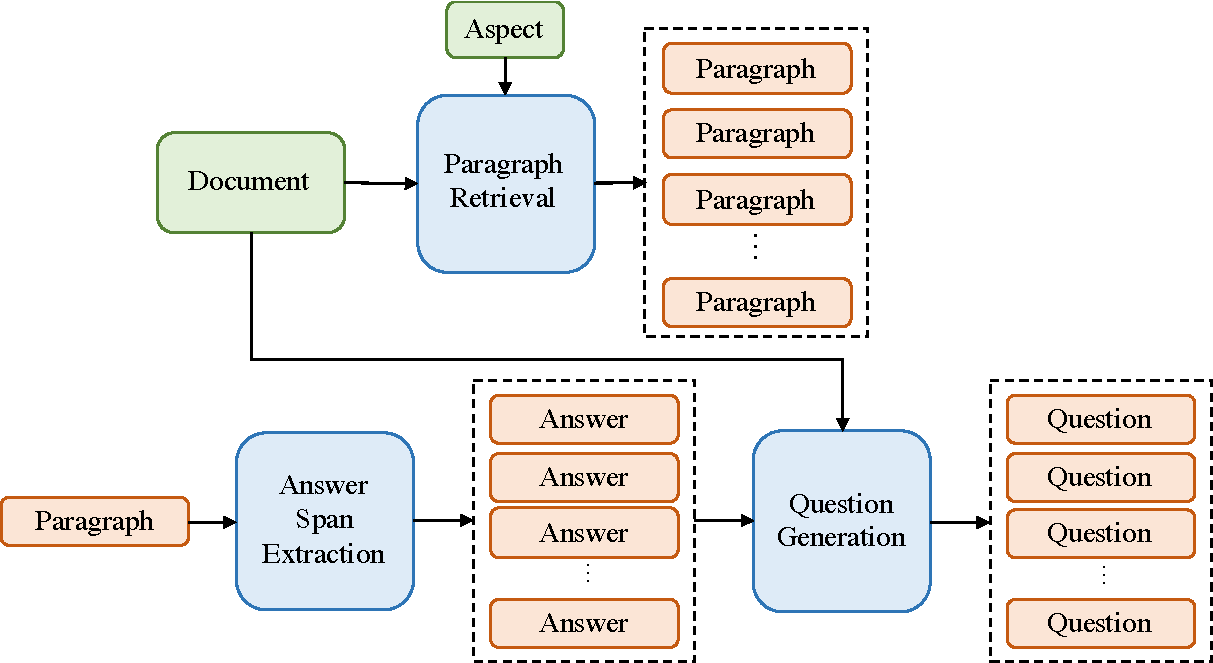
\includegraphics[width=0.45\textwidth]{pic/pipeline.pdf}
        \caption{\label{fig:pipeline} An overview of the pipeline process by which we generate QA pairs from the document. It consists of the feeding input data shown in blue blocks, the retrieval module, answer extraction module, and question generation module which are blocked in orange, and the intermediate and final results in green blocks.}
    \end{center}
\end{figure}

In the experiment, we use different combinations of the methods mentioned in each step since some methods may be more compatible with each other.

\subsection{Filtering Method}
In the task we proposed, the basic evaluation units are questions and answers, but in the ``Paragraph Retrieval'' step, we take the paragraphs as units to calculate the relevance between it and the aspect, which is a relatively simple process. It's easy for us to omit a paragraph that is related to the aspect but not highly related or generates irrelevant QA pairs in a relevant paragraph with this method. We propose a solution to this problem in this subsection.

The process of filtering method is shown in Figure \ref{fig:filtering}. In the filtering method, we choose all paragraphs in the document in the ``Paragraph Retrieval'' step and generate the QA pairs in the same way as Section \ref{sec:pipeline}. The difference is that there exists a filtering process after QA pairs are generated, we omit QA pairs that are not relevant to the aspect. In this case, QA pairs related to the aspect is not limited to certain paragraphs.

\begin{figure}[th]
    \begin{center}
    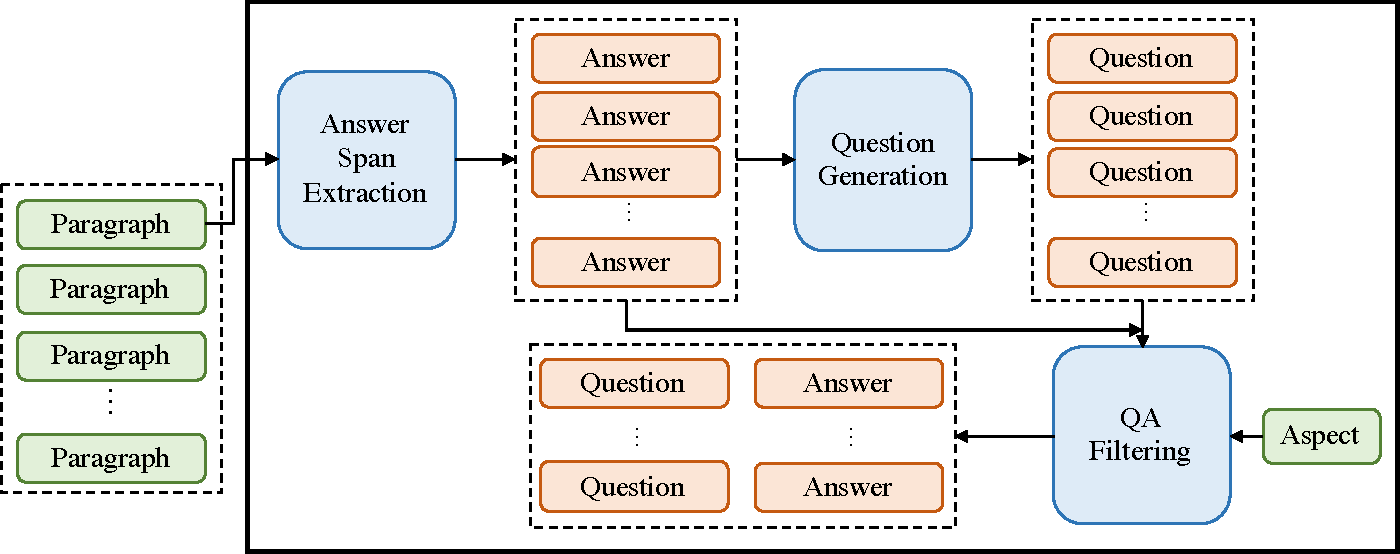
\includegraphics[width=0.45\textwidth]{pic/filtering.pdf}
        \caption{\label{fig:filtering} An overview of the filtering process by which we generate QA pairs from the document. Note that only one paragraph is blocked for clarity.}
    \end{center}
\end{figure}

We use a two-class sequence classifier as the filter. 
The filter takes the aspect, the answer and the question as the input and outputs a Boolean value as the judgment of whether the QA pair is relevant to the aspect. 
To make a better distinction between different segments of the input sequence, we add ``[SEP]'' tokens between different parts.

%\subsection{Joint Model: AspectQAG}
%% Inspired by the pre-trained language model UNILM~\cite{dong2019unified} which shares the Transformer~\cite{vaswani2017attention} concerning bidirectional LM, unidirectional LM, and sequence-to-sequence LM, we fine-tune our AspectQAG containing all of these LMs which is shown as Figure \ref{fig:joint}.
%
%Sharing parameters in close tasks is an effective method in Deep Learning. In this task, the embedding for paragraph and hint can be reused in answer extraction and question generation, and we proposed a joint model to reuse this embedding. The proposed model is called ``AspectQAG'', we show the architecture of the model in Figure~\ref{fig:joint}.
%
%\begin{figure}[th]
%    \begin{center}
%    \includegraphics[width=0.5\textwidth]{pic/joint-2.eps}
%        \caption{\label{fig:joint} An overview of AspectQAG. We pack the segments of paragraphs and hint together for simplicity because they have the same LM structure. There is a [SEP] token between the two segments. For Classifier Loss, we only consider the paragraph segment in $PH$. Same as UNILM, we use the self-attention mask to control the access to context for each token.}
%    \end{center}
%\end{figure}
%
%% As a joint model, AspectQAG is trained with two losses: the classifier loss for answer extraction and the generation loss for question generation. At test time, AspectQAG can extract answers with the input of paragraph and hint first, and then generate questions with the input of paragraph, hint and extracted answers.
%
%During training time, the input of AspectQAG is a sequence of tokens which consists of three parts: the segments of the paragraph and hint ($S_{PH}$), the segment of the answer ($S_{A}$) and the segment of the question ($S_{Q}$). 
%Training loss of the joint model has two major components, they are the classifier loss for answer extraction and the generation loss for question generation.
%% This joint model realizes the answer extraction and question generation at the same time. The details are as follows.
%
%\paragraph{Paragraph Retrieval.} We add irrelevant (paragraph, hint) pairs into the training data, the ground truth answers and questions of these irrelevant pairs are empty. The proportion of relevant and irrelevant (paragraph, hint) pairs is 5:1.
%
%\paragraph{Answer Extraction.} The contradiction between answer extraction and question generation is that the former does not take answers as input, but the latter requires it. Our solution is to mask the attention of the $S_{A}$ for $S_{PH}$ and take the transformer output of $S_{PH}$ to train the classifier. The output of the paragraph segment will go through a linear layer to give predict the label of each token in the paragraph among 'O', 'B', and 'I' (Note that the hint is documented independent, so we only mark the labels in paragraph area). We obtain classifier loss by calculating the cross entropy of the prediction and ground truth labeled sequence.
%
%% As shown in Figure \ref{fig:joint}(b), this module is related to the area of $S_{PH}$ 
%% %which is shown in Figure \ref{fig:joint}(b).
%% where only the paragraph and hint are available.
%% We choose the unidirectional LM to support the sequence labeling for answer span extraction with the label of `O', `B' and `I'.
%% Note that the hint is documented independently, so we only mark the labels in the paragraph area.
%
%\paragraph{Question Generation.} During question generation, the answer segment $S_A$ is considered as the source sequence together with $S_{PH}$, and the question segment $S_Q$ is regarded as the target sequence. We randomly mask 80\% tokens in the question segment $S_Q$ and learn to predict the masked token during training time. Since the output sequence is unknown at test time, we follow the decoder of the seq2seq structure and use a left-to-right attention mask in segment $S_Q$. We take the loss of masked token prediction as the generation loss. 
%
%% In this module, the answer segment $S_A$ is considered as the source sequence together with $S_{PH}$, and the question segment $S_Q$ is regarded as the target sequence.
%% Because $S_A$ is invisible in answer extraction module, there is a bidirectional LM for $S_A$ but a left-to-right unidirectional LM between $S_{PH}$ and $S_A$.
%% To follow the principle of sequence-to-sequence structure, there is a left-to-right unidirectional LM which allows the context of the to-be-predicted token in $S_Q$ contains all the tokens in $S_{HP}$ and $S_A$ and the tokens on its left.
%
%For overall training, we calculate the final loss as the synthesis of the answer extraction and question generation. We add two losses at a certain ratio as the final loss for training.
%\begin{equation}
%    Loss = Loss_{classifier} + \lambda \cdot Loss_{generation}
%\end{equation}
%
%% \SY{loss function}
%
%At test time, we take all paragraphs in the input document as the input and generate QA pairs in two steps. The first step is to extract answer spans with the classifier taken paragraph and hint as input. If the result is an empty set, we consider the input paragraph and hint as irrelevant, otherwise, we continue to the second step and generate questions with the generation component taken paragraph, hint and the extracted answers as input.